\documentclass{article}
%%%%%%%%%%%%%%%%%%%%%%%%%%%%%%%%%%%%%%%%%%%%%%%%%%%%%%%%%%%%%%%%%%%%%%%%%%%%%%%%%%%%%%%%%%%%%%%%%%%%%%%%%%%%%%%%%%%%%%%%%%%
\usepackage[scientific-notation=true]{siunitx} % Provides the \SI{}{} and \si{} command for typesetting SI units
\usepackage{graphicx} % Required for the inclusion of images
\graphicspath{{images/}}
\usepackage{natbib} % Required to change bibliography style to APA
\usepackage{amsmath} % Required for some math elements 
\usepackage[spanish,activeacute]{babel}
\usepackage{float}
\usepackage[table]{xcolor}
\usepackage[table]{xcolor}
\usepackage{anysize}
\usepackage{caption}
\usepackage{subcaption}
\usepackage{pdfpages}%insertar pdf
\marginsize{1in}{1in}{1in}{1in} 
\usepackage{enumerate}
\usepackage[utf8]{inputenc}
\usepackage{wrapfig}
\usepackage{multirow, array}
\usepackage{graphicx}
\usepackage{flushend}
\usepackage[utf8]{inputenc}
%%%%%%%%%%%%%%%%%%%%%%%%%%%%%%%%%%%%%%%%%%%%%%%%%%%%%%%%%%%%%%%%%%%%%%%%%%%%%%%%%%%%%%%%%%%%%%%%%%%%%%%%%%%%%%%%%%%%%%%%%%%%%%
\newcommand{\HRule}{\rule{\linewidth}{0.5mm}}
\setlength\parindent{0pt} % Removes all indentation from paragraphs

\renewcommand{\labelenumi}{\alph{enumi}.} % Make numbering in the enumerate environment by letter rather than number (e.g. section 6)

\newcolumntype{a}{>{\columncolor[gray]{0.9}}c}
%%%%%%%%%%%%%%%%%%%%%%%%%%%%%%%%%%%%%%%%%%%%%%%%%%%%%%%%%%%%%%%%%%%%%%%%%%%%%%%
\begin{document}
%%%%%%%%%%%%%%%%%%%%%
%PORTADA
%%%%%%%%%%%%%%%%%%%%%
\begin{center}

\includegraphics[width=0.3\textwidth]{Escudo_Unison.png}~\\[1cm]

\textsc{\LARGE Universidad de Sonora}\\[0.1cm]
\textsc{División de Ciencias Exactas y Naturales}\\[0.1cm]
\textsc{Departamento de Física}\\[1.5cm]
%\includegraphics[width=0.3\textwidth]{.png}~\\[1cm]

\HRule \\[0.4cm]
\textsc{Actividad 7: Sistema de Masas con Oscilaciones no Lineales y Forzadas}\\[0.1cm]
\textsc{Física Computacional I \\[0.1cm]}
\HRule \\[1.5cm]

\textsc{Rolando Abdel Fimbres Grijalva \\[1.0cm]}

\vfill
\textsc{14 de abril de 2018\\[0.1cm]}
\pagenumbering{gobble}
\end{center}
%%%%%%%%%%%%%%%%%%%%%%%%%%%%%%%%%%%%%%%%%%%%
\newpage
\pagenumbering{arabic}

\section{Introducción}
En la actividad se estudió la modelación de un fenómeno físico. Con la ayuda del lenguaje de programación Python. El caso de estudio fue un sistema de resortes acoplado. El método con el que podremos determinar la solución de éste sistema es mediante la aplicación de métodos numéricos. De esa forma podremos acercarnos a una solución más exacta.\\ 
A continuación se escribirá una breve síntesis del artículo de Temple H. Fay y Sarah Duncan Graham. También se añadirán imágenes de los códigos utilizados para resolver las problemáticas.
\section{Síntesis}
Estudiar las ecuaciones diferenciales es algo muy importante ya que para todo estudiante de física, la gran mayoría de fenómenos pueden modelarse gracias a ellas. Es muy importante contar con la ayuda de una herramienta que nos ayude para su solución. En éste caso sería la programación utilizando métodos numéricos.\\
En el artículo podemos observar que se desarrolla un problema por así llamar "clásico". Éste es el de dos resortes con dos pesas que se encuentran colgadas del techo. Según el artículo debemos recurrir a la Ley de Hooke, pues las fuerzas restaurativas se comportan de acuerdo a ésta ley. El problema se maneja con la ayuda de dos ecuaciones diferenciales lineales de segundo orden acopladas. Al nosotros diferenciar y sustituir valores, observamos que el movimiento de cada pesa es determinado por una ecuación diferencial de cuarto orden.\\
\subsection{El Resorte Acoplado}
El modelo consta de dos resortes y dos pesas que se cuelgan del techo. debemos tomar en cuenta que cada resorte cuenta con una constante en este caso: $k_{1}$ y $k_{2}$. Y masas: $m_{1}$ y $m_{2}$.
\subsection{Ley de Hooke}
Asumiremos que existen en el caso oscilaciones pequeñas. Las fuerzas restaurativas resultarían: $-k_{1}l_{1}$ y $-k_{2}l_{2}$ en donde $l_{1}$ y $l_{2}$ son las compresiones o elongamientos de los resortes. Debido a que la masa superior lleva ambos resortes, hay dos fuerzas de restauración actuando.\\
Tenemos presente una fuerza de restauración hacia arriba $k_{1}l_{1}$ ejercida por el elongamiento del primer resorte. Después del segundo una con forma $k_{2}(x_{2}-x_{1})$. La segunda masa solo cuenta con la fuerza de restauración del segundo resorte. Asumiendo que no hay fuerzas de amortiguamiento presentes, las Leyes de Newton que representan a los movimientos son:\\
\begin{center}
$m_{1}\ddot{x_{1}}=-k_{1}x_{1}-k_{2}(x_{1}-x_{2})$\\
$m_{2}\ddot{x_{2}}=-k_{2}(x_2-x_1)$\\
\end{center}
Para encontrar una ecuación para $x_{1}$ y $x_{2}$ que no dependen una de otra se resuelve la ecuación de $x_{2}$ y se sustituye en la de $x_{1}$, obteniendo las ecuaciones:\\
\begin{center}
$m_{1}m_{2}x_{1}^{(4)}+(m_{2}k_{1}+k_{2}(m_{1}+m_{2}))\ddot{x_{1}}+k_{1}k_{2}x_{1}=0$\\
$m_{1}m_{2}x_{2}^{(4)}+(m_{2}k_{1}+k_{2}(m_{1}+m_{2}))\ddot{x_{2}}+k_{1}k_{2}x_{2}=0$

\end{center}
\subsection{Añadiendo no linealidad}
Al asumir que las fuerzas restauradoras son no lineales y tienen la forma $-kx+\mu x^{3}$, entonces las ecuaciones quedan:\\
\begin{center}
$m_{1}\ddot{x_{1}}=-\delta_{1}\dot{x_{1}}-k_{1}x_{1}+\mu_{1}x_{1}^{3}-k_{2}(x_{1}-x_{2})+\mu_{2}(x_{2}-x_{1})^{3}$\\
$m_{2}\ddot{x_{2}}=-\delta_{2}\dot{x_{2}}-k_{2}(x_{2}-x_{1})+\mu_{2}(x_{2}-x_{1})^{3}$\\
\end{center}
La solución se complica mucho más que en los casos de linealidad.\\
\begin{figure}[H]
	\centering
    \includegraphics[width=\linewidth]{vf_31.png}\\
\end{figure}
\textbf{Ejemplo 3.1}: Asuma que $m_{1}=m_{2}=1$. Describe el movimiento para resortes con constantes $k_{1}=0.4$ y $k_{2}=1.808$, coeficientes de amortiguamiento $\delta_{1}=0$ y $\delta_{2}=0$, coeficientes de no linealidad $\mu_{1}=-1/6$ y $\mu_{2}=-1/10$, y con condiciones iniciales $(x_{1}(0),\dot{x_{1}}(0),x_{2}(0),\dot{x_{2}}(0))=(1,0,-1/2,0)$.\\
Debido a la falta de amortiguamiento, existe un comportamiento oscilatorio que aparenta periodicidad.\\
\begin{figure}[H]
	\centering
    \includegraphics[width=\linewidth]{ej31.png}
\end{figure}
De este modo obtenemos los resultados siguientes.
\begin{figure}[H]
	\centering
    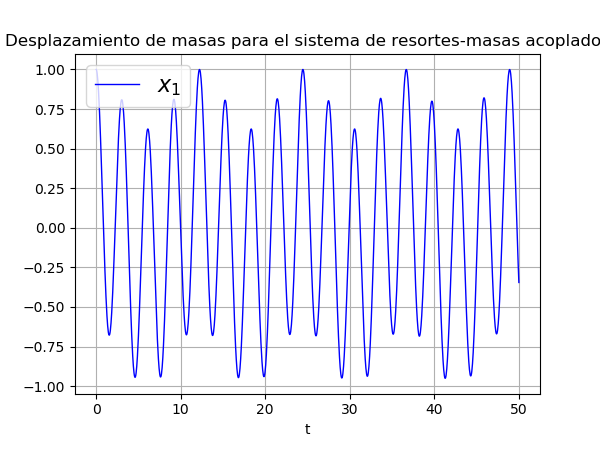
\includegraphics[width=\linewidth]{31_d1.png}
\end{figure}
\begin{figure}[H]
	\centering
    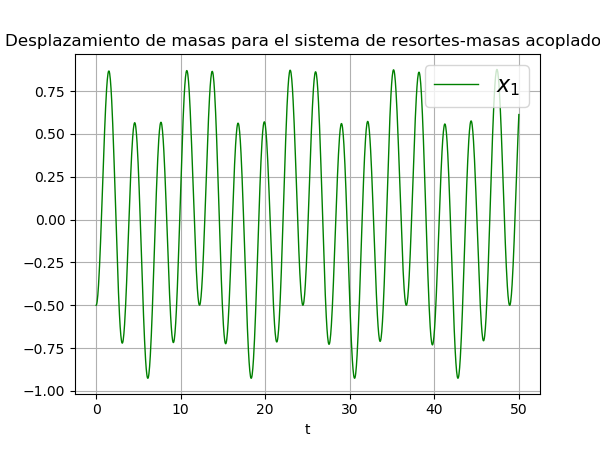
\includegraphics[width=\linewidth]{31_d2.png}
\end{figure}
\begin{figure}[H]
	\centering
    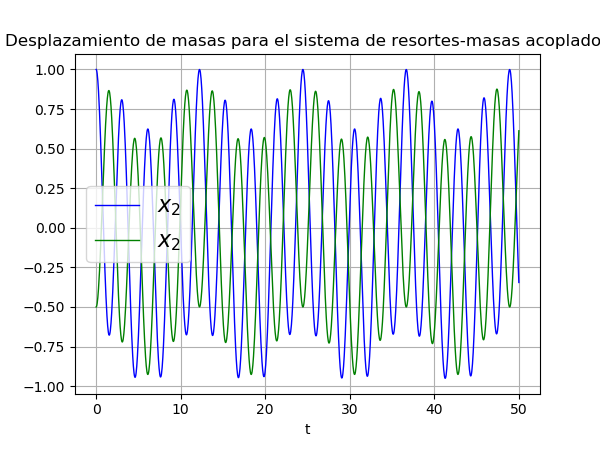
\includegraphics[width=\linewidth]{31_d12.png}
\end{figure}
\begin{figure}[H]
	\centering
    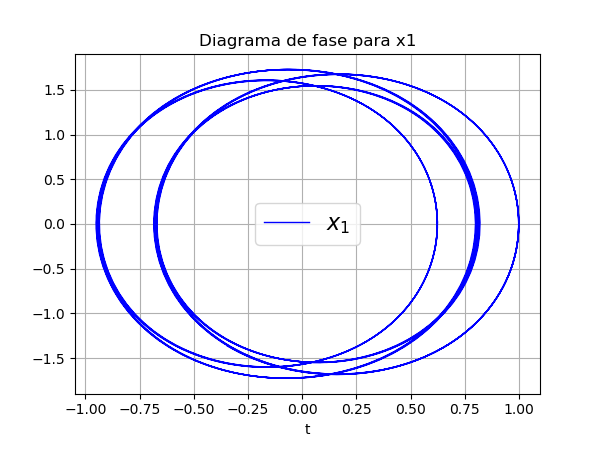
\includegraphics[width=\linewidth]{31_f1.png}
\end{figure}
\begin{figure}[H]
	\centering
    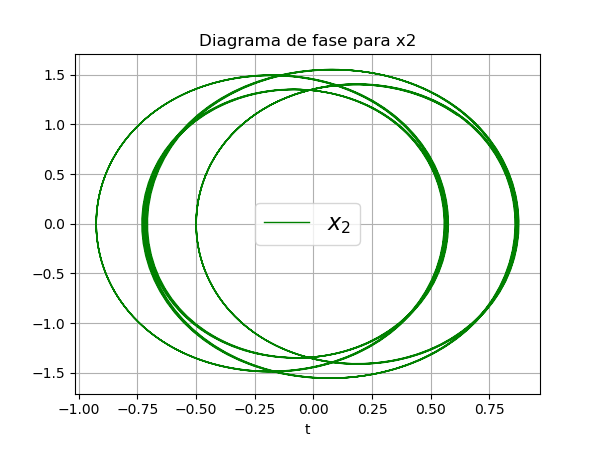
\includegraphics[width=\linewidth]{31_f2.png}
\end{figure}
\begin{figure}[H]
	\centering
    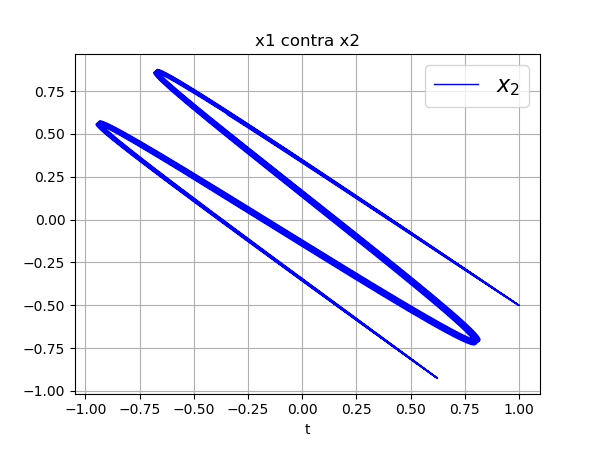
\includegraphics[width=\linewidth]{31_v.png}
\end{figure}
\textbf{Ejemplo 3.2}: Asuma que $m_{1}=m_{2}=1$. Describe el movimiento para resortes constantes $k_{1}=0.4$ y $k_{2}=1.808$, coeficientes de amortiguamiento $\delta_{1}=0$ y $\delta_{2}=0$, coeficientes de no linealidad $\mu_{1}=-1/6$ y $\mu_{2}=-1/10$, y con condiciones iniciales $(x_{1}(0),\dot{x_{1}}(0),x_{2}(0),\dot{x_{2}}(0))=(-0.5,1/2,3.001,5.9)$.\\
\begin{figure}[H]
	\centering
    \includegraphics[width=\linewidth]{ej32.png}
\end{figure}
Obteniendo los resultados:\\
\begin{figure}[H]
	\centering
    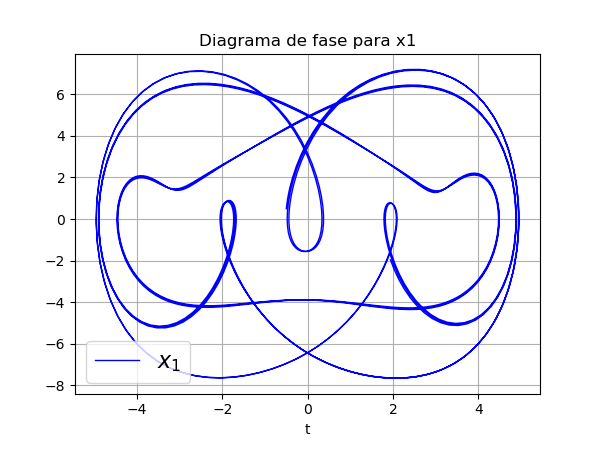
\includegraphics[width=\linewidth]{32_f1.png}
\end{figure}
\begin{figure}[H]
	\centering
    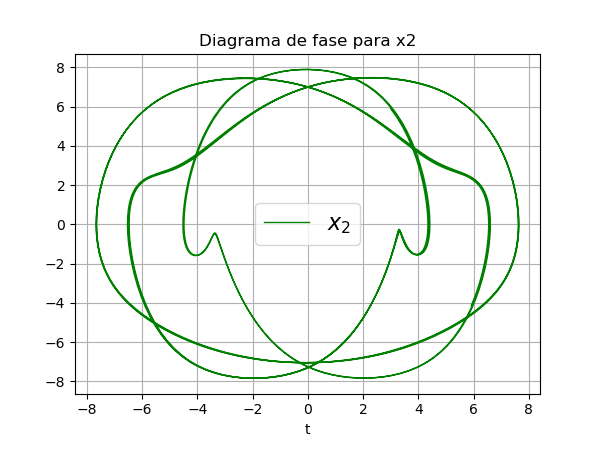
\includegraphics[width=\linewidth]{32_f2.png}
\end{figure}
\begin{figure}[H]
	\centering
    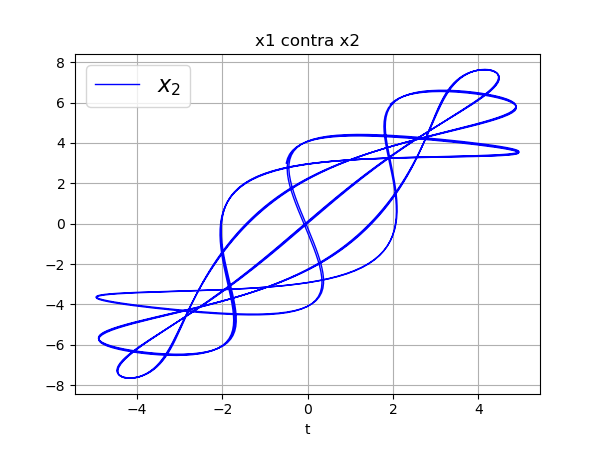
\includegraphics[width=\linewidth]{32_v.png}
\end{figure}
\textbf{Ejemplo 3.3}: Asuma que $m_{1}=m_{2}=1$. Describe el movimiento para resortes constantes $k_{1}=0.4$ y $k_{2}=1.808$, coeficientes de amortiguamiento $\delta_{1}=0$ y $\delta_{2}=0$, coeficientes de no linealidad $\mu_{1}=-1/6$ y $\mu_{2}=-1/10$, y con condiciones iniciales $(x_{1}(0),\dot{x_{1}}(0),x_{2}(0),\dot{x_{2}}(0))=(-0.6,1/2,3.001,5.9)$.\\
\begin{figure}[H]
	\centering
    \includegraphics[width=\linewidth]{ej33.png}
\end{figure}
Dando los siguientes resultados:\\
\begin{figure}[H]
	\centering
    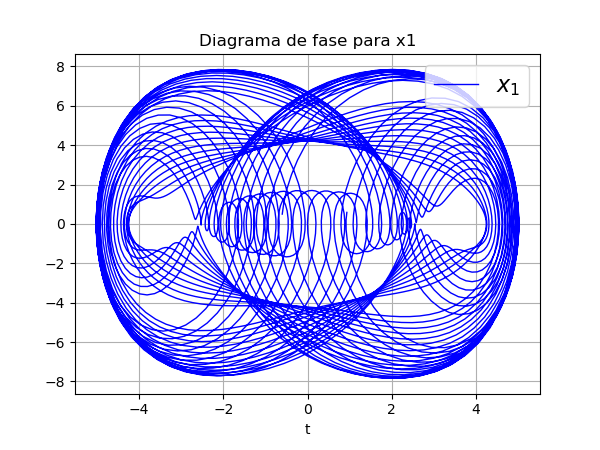
\includegraphics[width=\linewidth]{33_f1.png}
\end{figure}
\begin{figure}[H]
	\centering
    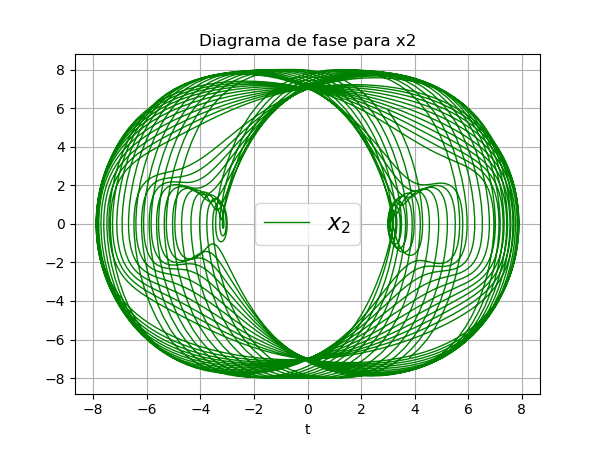
\includegraphics[width=\linewidth]{33_f2.png}
\end{figure}
\begin{figure}[H]
	\centering
    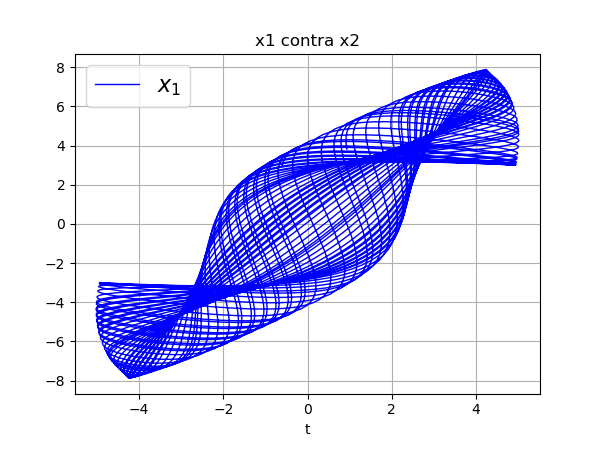
\includegraphics[width=\linewidth]{33_v.png}
\end{figure}
\subsection{Añadiendo forzamiento}
Para agregar una fuerza externa al sistema se aplica una fuerza con forma senoidal: $F\cos(wt)$. Nuestras ecuaciones quedan:\\
\begin{center}
$m_{1}\ddot{x_{1}}=-\delta_{1}\dot{x_{1}}-k_{1}x_{1}+\mu_{1}x_{1}^{3}-k_{2}(x_{1}-x_{2})+\mu_{2}(x_{2}-x_{1})^{3}+F_{1}\cos(w_{1}t)$\\
$m_{2}\ddot{x_{2}}=-\delta_{2}\dot{x_{2}}-k_{2}(x_{2}-x_{1})+\mu_{2}(x_{2}-x_{1})^{3}+F_{2}\cos(w_{2}t)$\\
\end{center}
\textbf{Ejemplo 4.1}: Asuma $m_{1}=m_{2}=1$. Describe el movimiento con constantes $k_{1}=2/5$ y $k_{2}=1$, coeficientes de amortiguamiento $\delta_{1}=1/10$ y $\delta_{2}=1/5$, coeficientes de no linealidad $\mu_{1}=1/6$ y $\mu_{2}=1/10$, fuerzas de amplitud $F_{1}=1/3$ y $F_{2}=1/5$, frecuencias de forzamiento $w_{1}=1$ y $w_{2}=3/5$ y con condiciones iniciales $(x_{1}(0),\dot{x_{1}}(0),x_{2}(0),\dot{x_{2}}(0))=(0.7,0,0.1,0)$.\\
Modificamos el campo vectorial:\\
\begin{figure}[H]
	\centering
    \includegraphics[width=\linewidth]{cv41.png}
\end{figure}
\begin{figure}[H]
	\centering
    \includegraphics[width=\linewidth]{ej41.png}
\end{figure}
Obteniendo los resultados:\\
\begin{figure}[H]
	\centering
    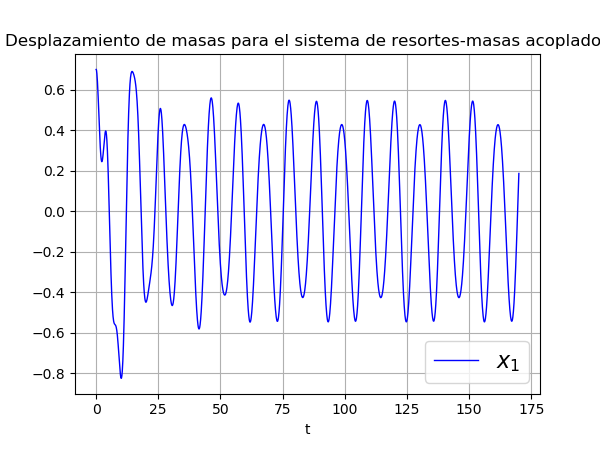
\includegraphics[width=\linewidth]{41_d1.png}
\end{figure}
\begin{figure}[H]
	\centering
    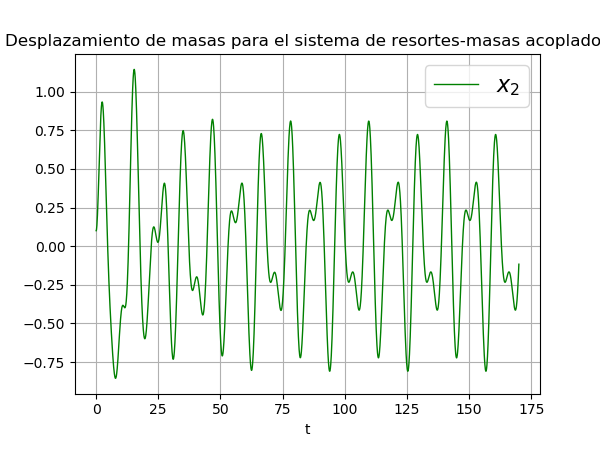
\includegraphics[width=\linewidth]{41_d2.png}
\end{figure}
\begin{figure}[H]
	\centering
    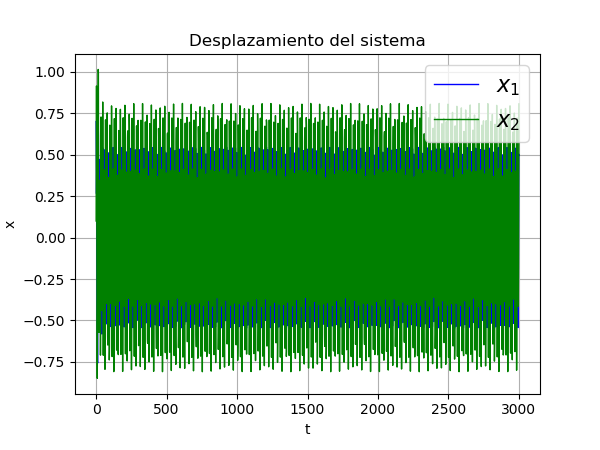
\includegraphics[width=\linewidth]{41_d12.png}
\end{figure}
\begin{figure}[H]
	\centering
    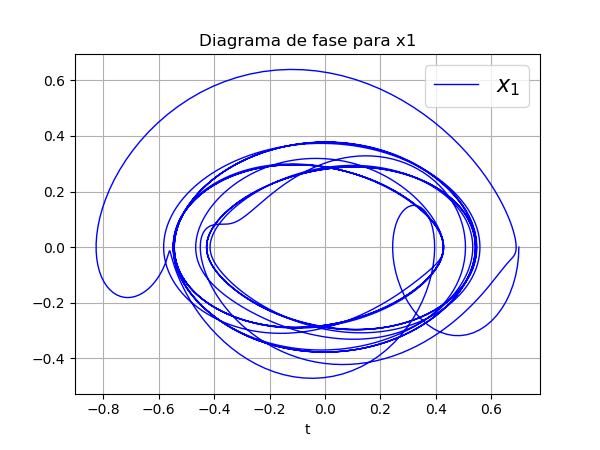
\includegraphics[width=\linewidth]{41_f1.png}
\end{figure}
\begin{figure}[H]
	\centering
    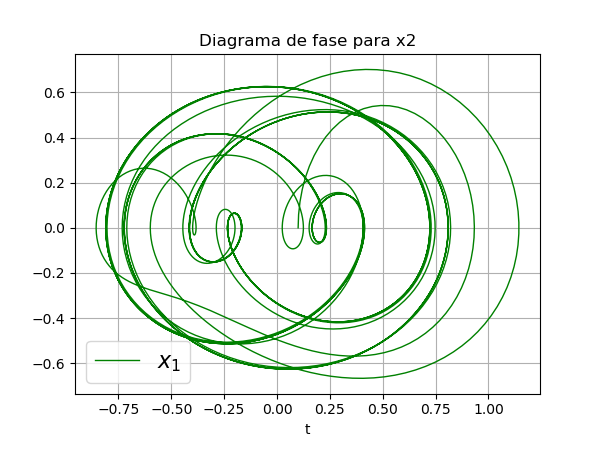
\includegraphics[width=\linewidth]{41_f2.png}
\end{figure}
\begin{figure}[H]
	\centering
    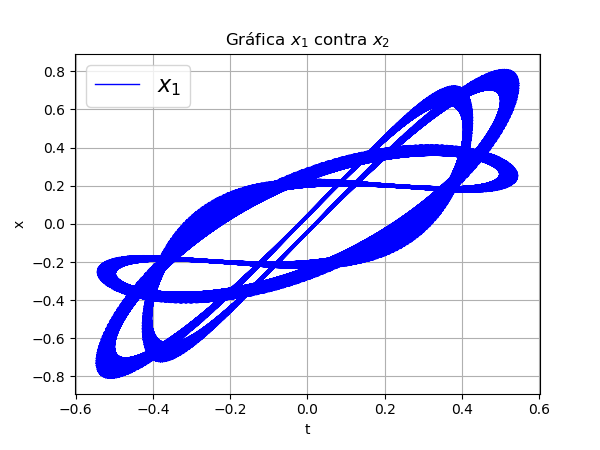
\includegraphics[width=\linewidth]{41_v.png}
\end{figure}
\begin{figure}[H]
	\centering
    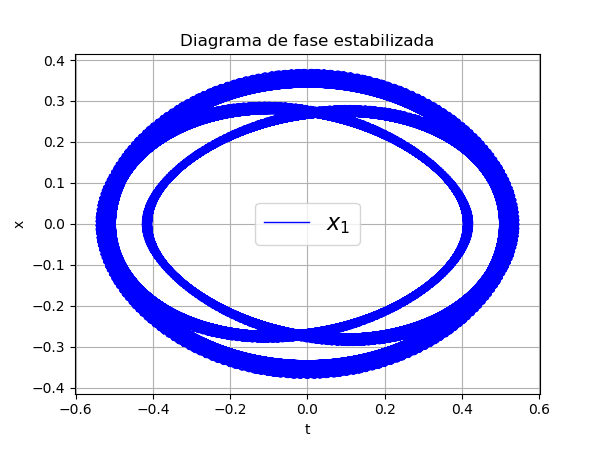
\includegraphics[width=\linewidth]{41_fe1.png}
\end{figure}
\begin{figure}[H]
	\centering
    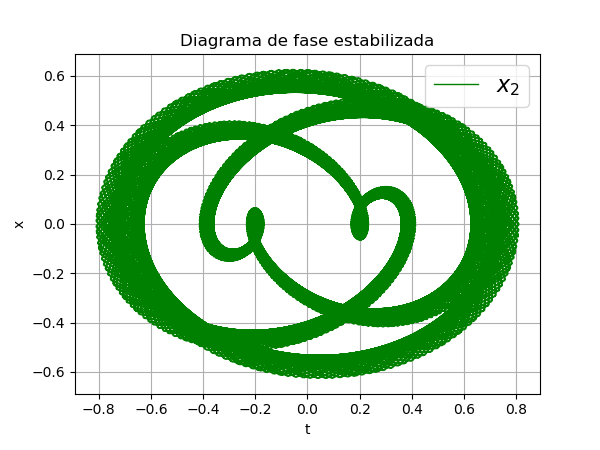
\includegraphics[width=\linewidth]{41_fe2.png}
\end{figure}
\section{Conclusiones}
Con esta actividad se aprendio a hacer un mejor uso de las herramientas para integracion numericas que ofrece python. Fue de gran ayuda porque permite tambien una visualizacion grafica de manera rapida.
\section{Bibliografia}
\begin{itemize}
\item Fay H., T., Duncan G. S., 2003., Coupled spring equations pp. 65-79. Int. J. Math. Educ. Sco. Technol.
\end{itemize}
\section{Apéndice}
1.¿Qué más te llama la atención de la actividad completa?\\
Que en el caso de fuerzas externas en el resorte debimos modificar el vector y ya no solo las condiciones iniciales.\\
2.¿De un sistema de masas acopladas como se trabaja en esta actividad, hubieras pensado que abre toda una nueva área de fenómenos no lineales?\\
No, no lo había pensado, sabía que habría un cambio, resultados nuevos, mas no una amplia gama de distintos resultados.\\
3.¿Qué propondrías para mejorar la actividad? ¿Te ha parecido interesante el reto?\\
Me parece bien, y no se me ocurre que se podría agregar.\\
4.¿Quisieras estudiar más éste tipo de fenómenos no lineales?\\
Si, pues considero que la mayoría de fenómenos son de éste tipo. No lineales.\\ 
\end{document}
